\documentclass[handout]{beamer}
\usepackage[utf8x]{inputenc}
\usepackage{ucs}
\usepackage{amsmath,tabularx}
\usetheme{Warsaw}
% \usecolortheme{crane}
% \usefonttheme{structurebold}
\newcolumntype{C}{>{\centering\arraybackslash}X}
\linespread{1}

\usepackage{subfigure}

\title[Hidden Structure]{\sc{ Combining latent topics with document attributes in text analysis}}
\author[NA]{Nelson Auner\\ 
 Prof. Matt Taddy\footnotemark \footnotetext[1]{Associate Professor of Econometrics and Statistics at Chicago Booth School of Business},
 Prof. Stephen Stigler\footnotemark \footnotetext[2]{Ernest DeWitt Burton Distinguished Service Professor at the Department of Statistics of the University of Chicago}
}





\institute[UChicago]{University of Chicago}
\date[13.05.2014]{May 13, 2014}

\usepackage{amsmath,supertabular,tabularx,graphicx,amssymb,amsfonts}
\usepackage{natbib,rotating}
%\usepackage{default}
\newcolumntype{Z}{>{\centering\arraybackslash}X}%



\renewcommand{\t}{\ensuremath{\theta}}
\renewcommand{\a}{\ensuremath{\alpha}}
\renewcommand{\b}{\ensuremath{\beta}}
\newcommand{\g}{\ensuremath{\gamma}}
\newcommand{\E}{\mathsf{E}}
\renewcommand{\d}{\ensuremath{\delta}}
\newcommand{\e}{\ensuremath{\epsilon}}
\newcommand{\s}{\sigma}
% \renewcommand{\S}{\Sigma}
\newcommand{\from}{\ensuremath{\leftarrow}}
\newcommand{\bm}{\mathbf}
\renewcommand{\l}{\lambda}
\newcommand{\dint}{\int\displaylimits}
\newcommand{\bx}{\mathbf x}
\newcommand{\by}{\mathbf y}
\newcommand{\be}{\pmb\e}
\renewcommand{\k}{\kappa}
\newcommand{\m}{\mu}
\newcommand{\A}{\ensuremath{\mathcal{A}}}
\newcommand{\B}{\ensuremath{\mathcal{B}}}
\newcommand{\sT}{\mathrm{T}}
\newcommand{\diag}{\mathrm{diag}}
\newcommand{\Tr}{\mathrm{Tr}}
\newcommand{\cov}{\mathbb{C}\mathrm{ov}~}
\newcommand{\var}{\mathbb{V}\mathrm{ar}~}


\AtBeginSection[]  % "Beamer, do the following at the start of every section"
{
\begin{frame}<beamer> 
\frametitle{Outline} % make a frame titled "Outline"
\tableofcontents[currentsection]  % show TOC and highlight current section
\end{frame}
}


\setcounter{footnote}{0}
\begin{document}

\begin{frame}
  \titlepage
\end{frame}

%%%%%%%%%%%%%%%%%%%

%\section{Text as Data }
%\subsection{Text}
%\subsection[Basic Structure]{Multinomial Models}
%\subsection{Metadata and Topic Models}
%\section{Cluster Membership Model}
%\subsection{Specification}
%\subsection[Parameter Estimation]{Estimation of Parameters}
%\subsection[Initialization]{Initialization of Cluster Membership
%\section{Application & Comparison with IRTM}
%\subsection{Congression Data}
%\subsection{Restaurant Reviews}
%\section{Extensions}
%\section*{References}

\begin{frame}
\frametitle{Motivation}
\pause
\begin{center}
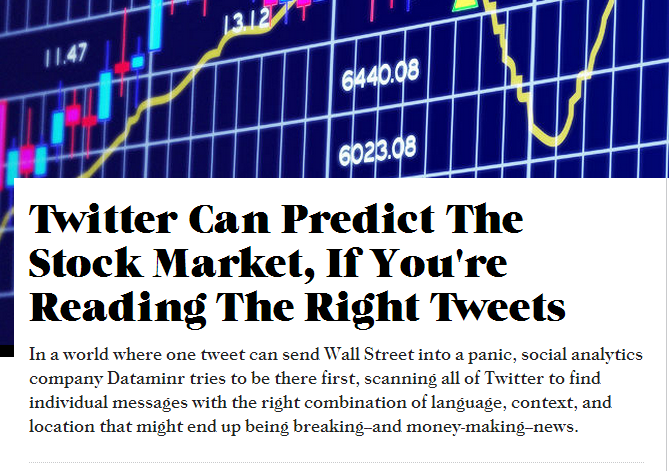
\includegraphics[height=.8\textheight]{Images/twitter_fastco.PNG}
\end{center}
\end{frame}

\begin{frame}
\frametitle{Motivation}
\pause
\begin{center}
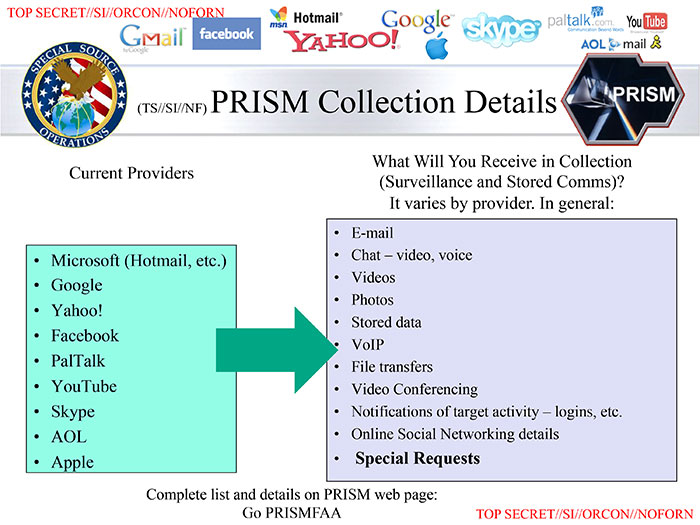
\includegraphics[height=.8\textheight]{Images/PRISM.jpg}
\end{center}
\end{frame}

\section{Text as Data }
\begin{frame}
 \frametitle{Text as Data}
 \begin{itemize}
\pause
\item A document is a collection of words or phrases.
\pause
\item Our datasets are collections of documents
\end{itemize}
\pause
\begin{table}[!hbpt]
\caption{What did homework consist of? } \label{tab:title}
\pause
\begin{center}
\begin{tabular} {c c}
\textbf{Document} & \textbf{Content} \\
\hline
1 & Some computation and formula proving, a lot of R code \\
2 & Problems, computation using R \\
3 & Some computations and writing R code\\
4 & Proofs, problems, and programming work \\
\end{tabular}
\end{center}
\end{table}
\end{frame}

\subsection[Basic Structure]{Multinomial Models}
\begin{frame}
\pause
\frametitle{Multinomial Models}
\begin{itemize}
\item If order doesn't matter, then we can treat each document as a "bag of words". 
\pause
\item The number of words can be modeled $\sim$ multinomial
\pause
\end{itemize}
\begin{table}[!hbpt]
\caption{Creating a word-count matrix from text}
\begin{center}
\resizebox{\textwidth}{!}{%
\begin{tabular}{ c |  c c c c c c c c c c c}
\hline
\textbf{Document} & Some & comp & formula & prov & R & code & use &
problem & writ & program & work \\
1 & 1 & 1 & 1 & 1 & 1 & 1 & 0 & 0 & 0 & 0 & 0 \\
2 & 0 & 1 & 0 & 0 & 1 & 0 & 1 & 1 & 0 & 0 & 0 \\
3 & 1 & 1 & 0 & 0 & 1 & 0 & 0 & 0 & 1 & 0 & 0\\
4 & 0 & 0 & 0 & 1 & 0 & 0 & 0 & 1 & 0 & 1 & 1\\
\hline
\end{tabular}}
\end{center}
\end{table} 
\end{frame}


\begin{frame}
\frametitle{A better model: Metadata}
\begin{itemize}
\item We would like to add structure to the model for inference or prediction
\pause
\item Metadata is data that accompanies a document
\pause
\end{itemize}
\begin{table}[!hbpt]
\caption{What did homework consist of?} \label{tab:title}
\pause
\begin{center}
\begin{tabular} {l l}
\textbf{Grade} & \textbf{Content} \\
\hline
A+ & Some computation and formula proving, a lot of R code \\
B & Problems, computation using R \\
B & Some computations and writing R code\\
C+ & Proofs, problems, and programming work \\  %something about R :P
\end{tabular}
\end{center}
\end{table}
\end{frame}



\subsection{Metadata and Computation}
\begin{frame}
\frametitle{Metadata and Computation}
\begin{itemize}
\pause
\item $n$ documents with metadata that takes $m$ discrete values:
\pause
\item Normally, $n >> m$
\pause
\item $\Rightarrow$ Collapse observations by outcome variables. 
\pause
\item Model as $m$ observations, instead of $n$
\end{itemize}
\pause
\begin{table}[!hbpt]
\begin{center}
\resizebox{\textwidth}{!}{%
\begin{tabular}{ l |  c c c c c c c c c c c}
\hline
\textbf{Document} & Some & comp & formula & prov & R & code & use &
problem & writ & program & work \\
A+ & 1 & 1 & 1 & 1 & 1 & 1 & 0 & 0 & 0 & 0 & 0 \\
B & 1 & 2 & 0 & 0 & 2 & 0 & 1 & 1 & 1 & 0 & 0 \\
C & 0 & 0 & 0 & 1 & 0 & 0 & 0 & 1 & 0 & 1 & 1\\
\hline
\end{tabular}}
\end{center}
\end{table} 
\pause
Reality: There are thousands of course reviews
\end{frame}


\subsection{Topic Models}
\begin{frame}
 \frametitle{Topic Models}
A topic is a distribution of words. \\
In a topic model, documents are made of a mixtures of topics. 

\begin{columns}
\column{.3\textwidth}
\begin{block}<2->{Running Topic}
Stride, Pacing, Stretch
\end{block}
\column{.3\textwidth}
\begin{block}<3->{Bike Topic}
Pedal, Helmet, Gears
\end{block}
\column{.3\textwidth}
\begin{block}<4->{Swimming}
Stroke, Air, Water
\end{block}
\end{columns}
\begin{itemize}
\item<5-> A book about triathalon training $\sim$ $\theta_1$ Running + $\theta_2$ Biking + $\theta_3$ Swimming
\item<6-> Problem: We can no longer collapse observations, must use all $n$ observations
\end{itemize}
\end{frame}



\section{Cluster Model}
\begin{frame}
 \frametitle{Cluster Model}
\begin{block}{Goal}<1->
\begin{itemize}
\item Want to use the Topic Model but incorporate Metadata
\item Also want computational ease
\end{itemize}
\end{block}

\begin{block}{Approach}<2->
\begin{itemize}
\item Restrict each document to only one topic $\Rightarrow$ "cluster"
\item Can collapse observations over unique (metadata, cluster) combination
\item $ x_{i} \sim MN(q_{ij},m_{ij})    ; ~~  q_{ij} = \frac{exp(\alpha_j + y_i \phi_j + u_i \Gamma_{kj})}{\sum_{l=1}^{p}{exp(\alpha_l+ y_i \phi_l + u_i \Gamma_{kl})}} $
\end{itemize}
\end{block}
\end{frame}

\subsection{Algorithm}
\begin{frame}
\frametitle{Algorithm for Cluster Membership Model with Gamma Lasso Penalty}
\begin{enumerate}
\def\labelenumi{\arabic{enumi}.}
\item<+->
 Initialize cluster membership $u_i$ for $i = 1, \dots, n$
\item<+->
  Determine parameters $\alpha_, \phi, \Gamma$ by fitting a multinomial
  regression on $y_i | x_i , u_i$ with a gamma lasso penalty (Taddy 2013)
\item<+->
 For each document $i$, determine new cluster $u_i$ membership as \\
  $argmax_{k = 1,..,K} \big[  \ell(u_i| \alpha, \phi, \Gamma) \big]$
\item<+->
 Check if current cluster assignment is different from previous cluster assignment , ($\textbf{u}^{(t)}  = \textbf{u}^{(t-1)}$).If so, return to step 2. If not, end algorithm.
\end{enumerate}
\end{frame}
%
%\subsection{Cluster Initialization}
%\begin{frame}
%\frametitle{How do we initialize the clusters?}
%\onslide<1->{We test three different approaches:}
%\begin{enumerate}
%\item<2-> Randomly assign each observation to a cluster 
%\item<3-> Group documents by k-means, then assign clusters 
%\item<4-> Regress metadata on text, then group residual's by k-means to clusters
%\end{enumerate}
%%\onslide<5->{We'll look at the efficacy of each apprach.}
%\end{frame}


\section{Application}

\begin{frame}
\frametitle{Congressional Speech and Restaurant Reviews}
\begin{itemize}
\item<+-> We apply the algorithm to two datasets:
	\begin{itemize} 
	\item Congressional Speech records (Gentzkow and Shapiro, 2010) 
	\item A corpus of restaurant reviews called we8there.
	\end{itemize}
\item<+-> Questions:
	\begin{itemize}
	\item Can this simple model capture the variation explained by a topic model?
	\item How does choice of cluster initialization affect the fit? 
	\end{itemize}
\end{itemize}
\end{frame}


\subsection{Congressional Speech Data}

\begin{frame}
\frametitle{An Example Cluster}
% latex table generated in R 3.0.2 by xtable 1.7-1 package
% Wed May 07 18:31:04 2014
\begin{center}
\small
\begin{tabular}{rll}
  \hline
 & term & loading \\ 
  \hline
1 & nation.oil.food & 20.09 \\ 
  2 & united.nation.oil & 12.09 \\ 
  3 & liberty.pursuit.happiness & 8.11 \\ 
  4 & life.liberty.pursuit & 8.11 \\ 
  5 & minority.women.owned & 6.73 \\ 
  6 & universal.health & 6.67 \\ 
  7 & white.care.act & 6.64 \\ 
  8 & ryan.white.care & 6.6 \\ 
  9 & universal.health.care & 5.99 \\ 
  10 & growth.job.creation & 5.39 \\ 
  11 & drilling.arctic.national & 5.3 \\ 
  12 & tax.relief.package & 5.29 \\ 
  13 & judge.john.robert & 5.26 \\ 
  14 & fre.enterprise & 5.07 \\ 
  15 & arctic.refuge & 4.93 \\ 
   \hline
\end{tabular}
\end{center}
\end{frame}


\begin{frame}
\frametitle{Comparison with the Topic Model}
Good news: We are able to recover similar topics with our model:
\begin{table}[!htbp]
\caption{Comparison of top word loadings on a stem-cell topic} \label{tab:title}
\centering
\begin{tabular}{  c  c }
Cluster Membership & Topic Model (LDA)* \\
\hline
umbilic.cord.blood & pluripotent.stem.cel \\
cord.blood.stem  & national.ad.campaign \\
blood.stem.cel   & cel.stem.cel \\
adult.stem.cel & stem.cel.line \\
\end{tabular}
\end{table}
*Results reported in Taddy (2012)
\end{frame}

\begin{frame}
\frametitle{Incorporating metadata: Congressional Speech} %Graph of first topic:
\begin{center}
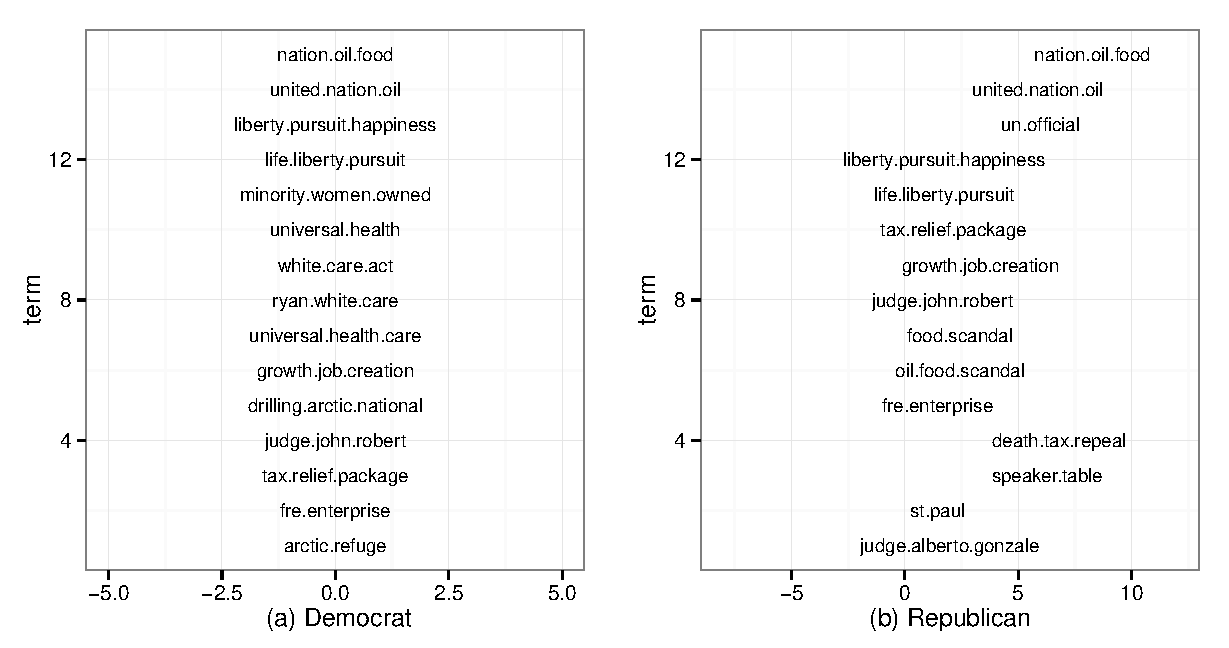
\includegraphics[width=1.1\textwidth]{Images/Blei_Changing_Loadings_GOP.pdf}
\end{center}
\end{frame}

\subsection{Restaurant Review Data}

\begin{frame}
\frametitle{Example Topic from Restaurant Review}

% latex table generated in R 3.0.2 by xtable 1.7-1 package
% Fri May 09 11:56:25 2014
\begin{center}
\small
\begin{tabular}{rll}
  \hline
 & term & loading \\ 
  \hline
1 & deep dish & 7.76 \\ 
  2 & italian beef & 7.07 \\ 
  3 & pizza like & 6.85 \\ 
  4 & style food & 6.69 \\ 
  5 & au jus & 6.33 \\ 
  6 & cut fri & 6.16 \\ 
  7 & just ok & 6.01 \\ 
  8 & great pizza & 5.96 \\ 
  9 & south side & 5.94 \\ 
  10 & pizza great & 5.82 \\ 
  11 & just over & 5.75 \\ 
  12 & took seat & 5.72 \\ 
  13 & golden brown & 5.61 \\ 
  14 & behind counter & 5.58 \\ 
  15 & got littl & 5.52 \\ 
   \hline
\end{tabular}
\end{center}
\end{frame}


\begin{frame}
\frametitle{Incorporating metadata: Restaurant Review} %Graph of first topic:
\begin{center}
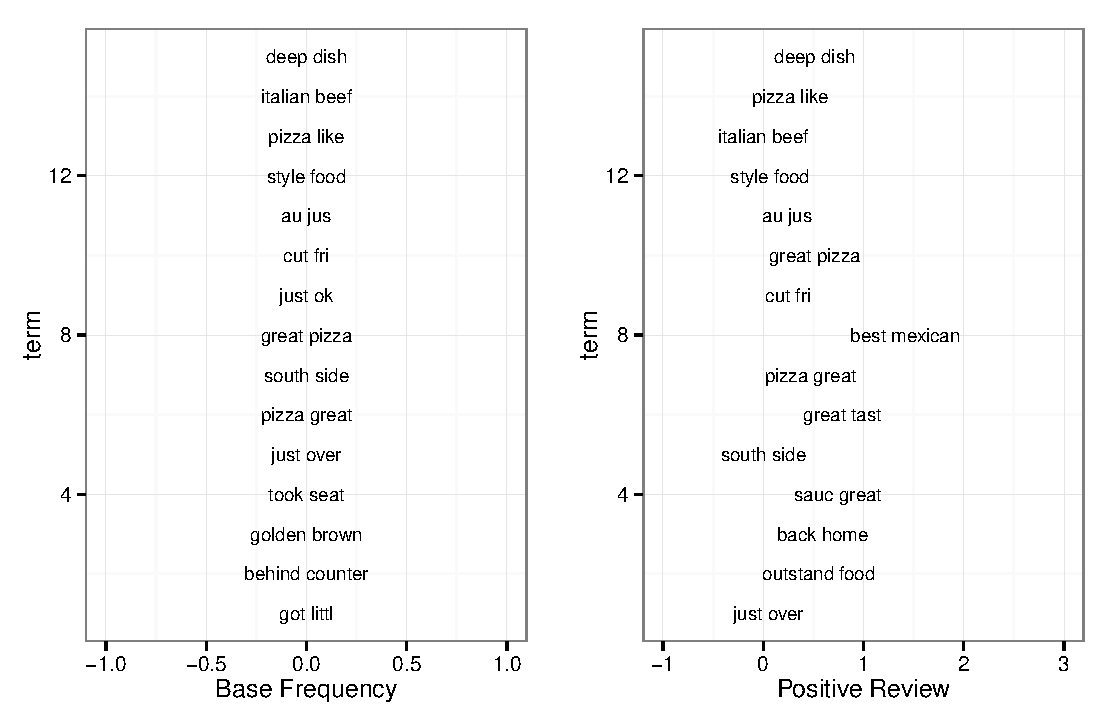
\includegraphics[width=1\textwidth]{Images/we8there_distortion.pdf}
\end{center}
\end{frame}
%
%\begin{frame}
%\frametitle{Evaluating Cluster Initialization}
%\begin{center}
%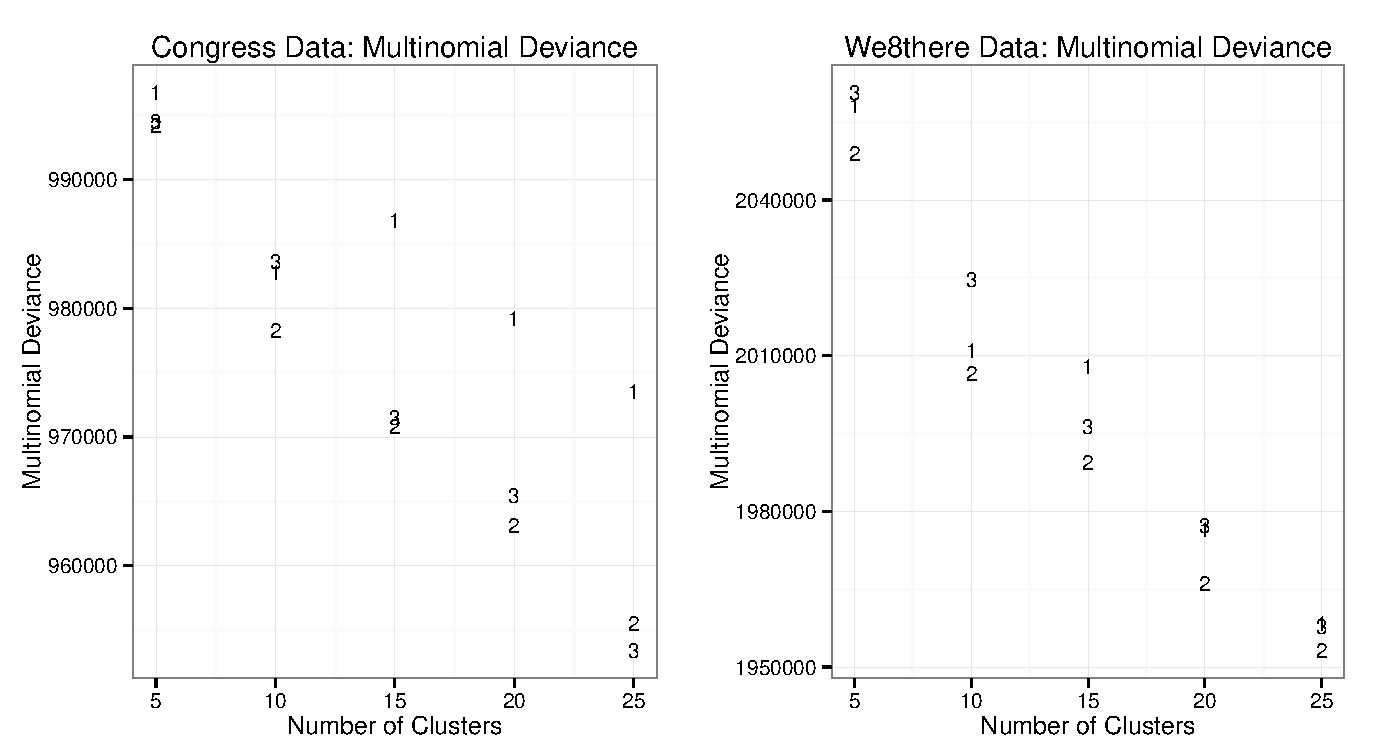
\includegraphics[width=1.05\textwidth]{Images/mdev_both.pdf}
%\end{center}
%\end{frame}

\section{Extensions}
\begin{frame}
\begin{enumerate}
\item<+-> Relationship Between Clusters and Metadata
\item<+-> Feature Allocations: Allow an obervation to be a member of multiple clusters
\item<+-> Prediction and Cross Validation
\end{enumerate}
\end{frame}

\begin{frame}
\frametitle{Imma Let you Finish, but the Dirichlet was the greatest prior of all time!}
\pause
\begin{center}
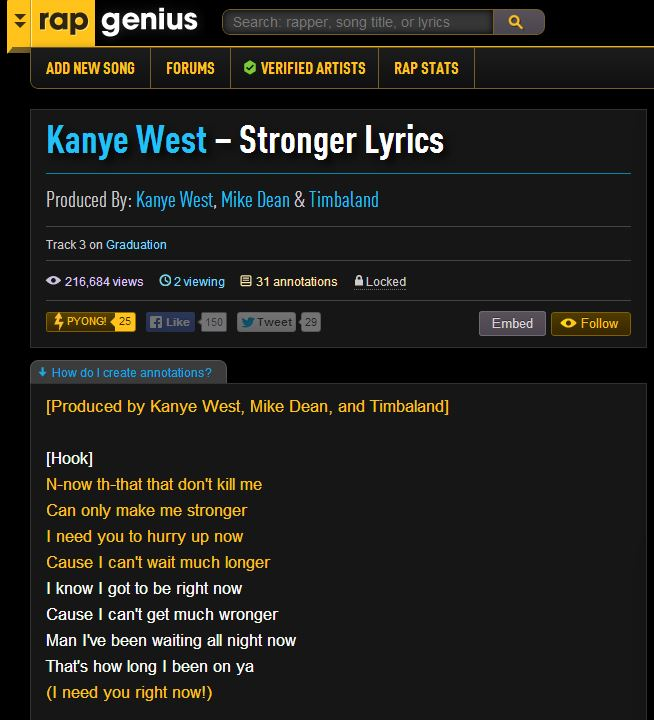
\includegraphics[height=1.0\textheight]{Images/lyrics_sample.png}
\end{center}
\end{frame}

\begin{frame}
\frametitle{Results}
\pause
% latex table generated in R 3.0.2 by xtable 1.7-1 package
% Mon May 12 22:33:48 2014
\begin{table}[ht]
\centering
\begin{tabular}{rll}
  \hline
 & term & loading \\ 
  \hline
1 & yeezus & 5.48 \\ 
  2 & constel & 3.79 \\ 
  3 & homm & 3.79 \\ 
  4 & preach & 3.79 \\ 
  5 & bound & 3.6 \\ 
  6 & thoma & 3.38 \\ 
  7 & thirti & 3.32 \\ 
  8 & rocka & 3.31 \\ 
  9 & rowland & 3.25 \\ 
  10 & jamaican & 3.23 \\ 
  11 & blocka & 3.22 \\ 
  12 & movement & 3.22 \\ 
  13 & unlik & 3.08 \\ 
  14 & yknow & 3.08 \\ 
   \hline
\end{tabular}
\end{table}
\end{frame}



\begin{frame}
\frametitle{Thank You}
\pause
\begin{center}
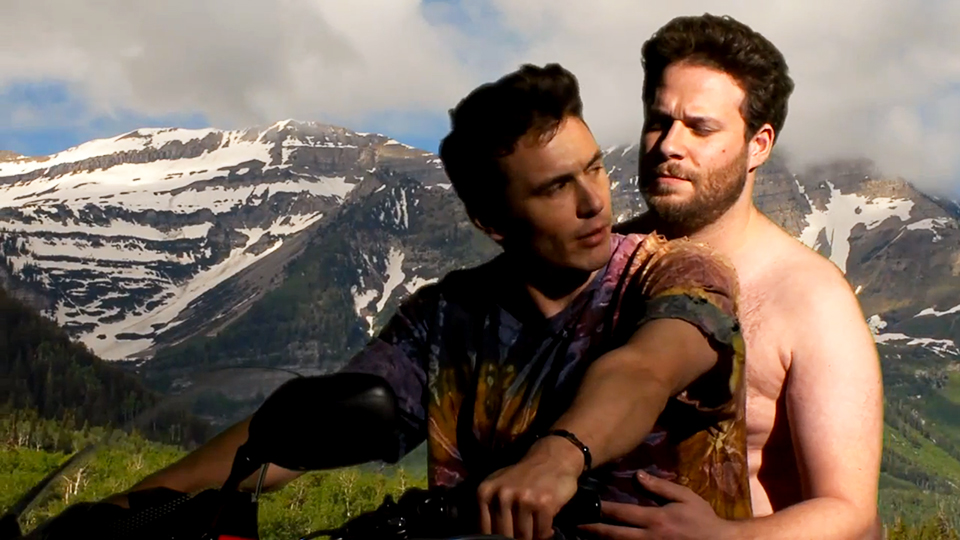
\includegraphics[height=1.0\textheight]{Images/rogen.jpg}
\end{center}
\end{frame}


\end{document}

